\documentclass[twoside,a4paper,openany,12pt]{article}

%%\documentclass[twoside,a4paper,12pt]{article}
%\documentclass[twoside,a4paper,openany,12pt]{report}

%% Document has convention that only first letter of chapters,
%% sections is capitalized. Do the same for automatic sections
\renewcommand\listfigurename{List of figures}
\renewcommand\listtablename{List of tables}
\newcommand{\secname}{Section}

%% Convenient way to specify margins
\usepackage[a4paper,top=2.5cm,bottom=2.5cm,inner=2.5cm,outer=2.5cm]{geometry}

%% Relative font sizes
\usepackage{relsize}

%% Use font with 8-bit encoding
\usepackage[T1]{fontenc}

%% Nicer fonts
\usepackage{pslatex}

\usepackage{linegoal}

\usepackage{array}
%\usepackage{longtable}
\usepackage{supertabular}

%% Color definitions
\usepackage{color}
\definecolor{MyLightRed}{rgb}{1,.8,.8}
\definecolor{MyCodeboxColor}{rgb}{.9,.9,.9}
\definecolor{MyLightBlue}{rgb}{.8,.8,1}
\definecolor{MyQuoteColor}{rgb}{0,.6,0}
\definecolor{MyLightMagenta}{rgb}{1,.2,1}
\definecolor{MyYellow}{rgb}{1,1,.6}

%% For landscape pages printed, but rotated on screen
\usepackage{pdflscape}

%% Allow linebreaks in all captions. Required by the \photoCredit
%% command.
\usepackage{caption}
% \captionsetup{justification=justified}

%% Including figures and other graphics
\usepackage{graphicx}
% \usepackage[rgb]{xcolor}
%% Rotated images etc
\usepackage{rotating}

%% Author-year citations
\usepackage[authoryear]{natbib}

%% Subfigure environment
\usepackage{subfigure}

%% Conditional sections
\usepackage{ifthen}

%% URLs
\usepackage[obeyspaces]{url}

%% SI units
\usepackage[abbreviations]{siunitx}

% Command to get a tilde which prints as an ASCII tilde in PDFs,
% needed to allow copying text and pasting into a command window or
% editor
\newcommand{\mytilde}{\texttildelow}

%% For tables align on decimal point
\usepackage{dcolumn}
\newcolumntype{d}{D{.}{.}{-1}} % centre on decimal place

%% Long tables
\usepackage{supertabular}

\usepackage{fancyhdr}

%% Alternative to verbatim. Can be used for defining new environments
\usepackage{fancyvrb}
%% A command to include Matlab files (verbatim). Surrounded with a
%% frame and smaller font size than normal. Must be defined before
%% underscore package because the custom command must be listed in
%% \UnderscoreCommands
\CustomVerbatimCommand{\IncludeMatlabFileVerb}{VerbatimInput}{frame=single,fontsize=\relsize{-1}}
\CustomVerbatimCommand{\IncludeShellFileVerb}{VerbatimInput}{frame=single,fontsize=\relsize{-1}}

%% Include Matlab file verbatim and attach it for the user to download.
\newcommand{\IncludeMatlabFile}[2]{\IncludeMatlabFileVerb{#1}%
  \attachfile[mimetype=text/plain,description=#2]{#1}}

%% Include shell file verbatim and attach it for the user to download.
\newcommand{\IncludeShellFile}[2]{\IncludeShellFileVerb{#1}%
  \attachfile[mimetype=text/plain,description=#2]{#1}}


%% Have floats on subsequent page, not miles away.
\usepackage{flafter}

\usepackage{marvosym} % for \Info
\usepackage{keystroke} % for keyboard symbols

\usepackage{abbrev}
\renewcommand{\abbrevname}{Abbreviations}
\renewcommand{\abbrevsection}[1]{\section*{#1}}
%% List of abbreviations. Include all useful ones. Those which are not
%% used are not included in the table.

\abbrev{\dtr}{DTR}{data terminal ready}
\abbrev{\eeprom}{EEPROM}{electrically erasable programmable read-only memory}
\abbrev{\esd}{ESD}{electro-static discharge}
\abbrev{\fet}{FET}{field-effect transistor}
\abbrev{\ic}{IC}{integrated circuit}
\abbrev{\itwoc}{I2C}{inter-integrated circuit (bus)}
\abbrev{\isp}{ISP}{in-circuit serial programmer (sometimes abbreviated as ICSP)}
\abbrev{\led}{LED}{light emitting diode}
\abbrev{\pcb}{PCB}{printed circuit board}
\abbrev{\psu}{PSU}{power supply unit}
\abbrev{\sd}{SD}{secure digital}
\abbrev{\soic}{SOIC}{small outline integrated circuit}
\abbrev{\ttl}{TTL}{transistor-transistor logic}
%% \url is already a command, use \URL for the abbreviation
\abbrev{\URL}{URL}{uniform resource locator}
\abbrev{\usb}{USB}{universal serial bus}



\input{gitlog}

% Load the underscore package as fixes the problem of copying and
% pasting text with underscores; previously underscores were converted
% to spaces, but they matter for code! Need to protect certain
% commands which take input which has underscores (see underscore
% package for details)
\newcommand{\UnderscoreCommands}{%
  \do\VerbatimInput
  \do\BVerbatimInput 
  \do\IncludeMatlabFileVerb
  \do\IncludeShellFileVerb
}
\usepackage[strings]{underscore}

%% Include these packages last!
% \usepackage[bookmarksnumbered=true,
% bookmarksopen=true,
% bookmarksopenlevel=0,
% unicode=true,
% pdftitle={AuroraWatchNet magnetometer manual}]{hyperref}

\usepackage[%
bookmarksnumbered=true,
bookmarksopen=true,
bookmarksopenlevel=0,
unicode=true,colorlinks=false,
allbordercolors={0 0 1},
pdfborderstyle={/S/U/W 1}]{hyperref}

% \usepackage[bookmarksnumbered=true,
% bookmarksopen=true,
% bookmarksopenlevel=0,
% colorlinks=true,
% linkcolor=blue,
% citecolor=blue,
% urlcolor=blue,
% unicode=true,
% pdftitle={AuroraWatchNet magnetometer manual}]{hyperref}

%% Have references to figures link to the top of the figure, not the
%% caption text.
\usepackage[all]{hypcap}

%% Attach files to PDF document. Set the default options we want.
\usepackage{attachfile2}
\attachfilesetup{icon=Paperclip}

%% Upright quotes, essential for quoting for Matlab code!
\usepackage{upquote}

\usepackage{pdfcomment}
\renewcommand{\insertabbrev}[2]{\pdftooltip{#1}{#2}}
\makeabbrev

%% A command for the return key
\newcommand{\myreturn}{%
  \keystroke{\includegraphics[width=1em]{images/return-symbol}}}

%% Change how subfigures are labelled
\makeatletter
\renewcommand{\@thesubfigure}{\figurename~\thefigure\alph{subfigure}: }
\renewcommand{\thesubfigure}{\alph{subfigure}}
%%%\renewcommand{\p@subfigure}{\alph{subfigure}}
\makeatother

% No indents at start of paragraph, but paragraphs have blank lines
% between them
\setlength{\parindent}{0pt}
\setlength{\parskip}{2ex} 


%% \filename allows for _ but otherwise is formatted identically to
%% code. If using tildes (~) then use \mytilde command, inside
%% \texttt. Use the url package's command to define this, that way
%% hyperref doesn't see it as a hyperref!
\DeclareUrlCommand\filename{\urlstyle{tt}}
\newcommand{\email}[1]{\href{mailto:#1}{#1}}
\newcommand{\ccBySaTwoUrl}{http://creativecommons.org/licenses/by-sa/2.0/}
\newcommand{\ccBySaThreeUrl}{http://creativecommons.org/licenses/by-sa/3.0/}

\newcommand{\ccBySaFourUrl}{http://creativecommons.org/licenses/by-sa/4.0/}
\newcommand{\ccByNcSaFourUrl}{%
  http://creativecommons.org/licenses/by-nc-sa/4.0/}

\newcommand{\ccBySaTwo}{\href{\ccBySaTwoUrl}{CC BY-SA 2.0}}
\newcommand{\ccBySaThree}{\href{\ccBySaThreeUrl}{CC BY-SA 3.0}}

\newcommand{\ccBySaFour}{\href{\ccBySaFourUrl}{CC BY-SA 4.0}}
\newcommand{\ccByNcSaFour}{\href{\ccByNcSaFourUrl}{CC BY-NC-SA 4.0}}

\newcommand{\rsyncUrl}{http://rsync.samba.org/}
%% Copyright, licence, URL.
\newcommand{\photoCredit}[4][]{\\ %
  \ifthenelse{\equal{#2}{}}{}{ \copyright~#2.}%
  \ifthenelse{\equal{#3}{}}{}{ #3.}%
  \ifthenelse{\equal{#4}{}}{}{ \href{#4}{#4}}}

%% Environment variables. Like \filename but prepends a $
\DeclareUrlCommand\envVar{\def\UrlLeft{\$}\urlstyle{tt}}
\DeclareUrlCommand\dosEnvVar{\def\UrlLeft{\%}\def\UrlRight{\%}\urlstyle{tt}}

\newcommand{\code}[1]{\texttt{#1}}
\newcommand{\username}[1]{\texttt{#1}}
\newcommand{\piUser}{\username{pi}}
\newcommand{\rootUser}{\username{root}}

%% Use for menu selections etc
\newcommand{\myquote}[1]{\textcolor{MyQuoteColor}{\textsl{#1}}}

%% Define our own keypress command, based on keystroke
\newcommand{\keypress}[1]{\keystroke{#1}}

%% Units
%%\newcommand{\units}[2]{\mbox{\ensuremath{#1}\,#2}}
%%\newcommand{\dB}[1]{\mbox{\ensuremath{#1}\,dB}}
\newcommand{\dB}[1]{\SI{#1}{dB}}
%%\newcommand{\inch}[1]{\mbox{\ensuremath{#1}''}}
\newcommand{\inch}[1]{\SI{#1}{''}}
\newcommand{\Hz}[1]{\SI{#1}{\hertz}}
\newcommand{\kHz}[1]{\SI{#1}{\kilo\hertz}}
\newcommand{\MHz}[1]{\SI{#1}{\mega\hertz}}
\newcommand{\volt}[1]{\SI{#1}{V}}
  \newcommand{\voltOLD}[1]{\mbox{\ensuremath{#1}\,V}}
\newcommand{\bit}[1]{\mbox{\ensuremath{#1}\,bit}}

%%\newcommand{\degrees}[1]{\ensuremath{#1^\circ}}

\renewcommand{\textohm}{\ensuremath{\Omega}}
\newcommand{\ohm}[1]{\SI{#1}{\ohm}}
\newcommand{\kohm}[1]{\SI{#1}{\kilo\ohm}}


\newcommand{\pF}[1]{\SI{#1}{\pico\farad}}
\newcommand{\nF}[1]{\SI{#1}{\nano\farad}}
\newcommand{\uF}[1]{\SI{#1}{\micro\farad}}

\newcommand{\uH}[1]{\SI{#1}{\micro\henry}}

\newcommand{\nT}[1]{\SI{#1}{\nano\tesla}}

\newcommand{\MB}[1]{\SI{#1}{\mega\byte}}
%% Some simple abbreviations  
\newcommand{\ie}{i.e.}
\newcommand{\eg}{e.g.}
\newcommand{\etal}{\latin{et al.}}
\newcommand{\etc}{etc.}

%% Have warnings printed in light red box, with each item using a
%% STOP sign as a bullet
\newenvironment{warninglist}{%
  \begin{list}{\Stopsign}{}}{%
    \end{list}}
\newcommand{\warningbox}[1]{\noindent%
  \colorbox{MyLightRed}{\parbox{\textwidth}{%
      \begin{warninglist}\item #1\end{warninglist}}} \newline}

%% Have help information printed in light blue box, with each item using an
%% information sign as a bullet
\newenvironment{helplist}{%
  \begin{list}{\Info}{}}{%
    \end{list}}
\newcommand{\helpbox}[1]{\noindent
  \colorbox{MyLightBlue}{\parbox[l]{\textwidth}{%
      \begin{helplist}\item #1\end{helplist}}} \newline}
\newcommand{\examplebox}[2][]{\noindent
  \colorbox{MyYellow}{\parbox[l]{\textwidth}{\ifthenelse{\equal{#1}{}}%
      {Example: }{#1}\vspace*{1ex} \newline %
      #2 %
      \vspace*{1ex}}} \newline}


%% Verbatim-like environment for code.
\DefineVerbatimEnvironment{Code}{Verbatim}%
{frame=single,commandchars=\\\{\}}
\DefineVerbatimEnvironment{Cmd}{Verbatim}%
{frame=single,framesep=5mm,commandchars=\\\{\}}
% {frame=single,label=\linuxLogo,framesep=5mm,commandchars=\\\{\}}
\DefineVerbatimEnvironment{LinuxCmd}{Verbatim}%
{frame=single,framesep=5mm,commandchars=\\\{\}}
% {frame=single,label=\linuxLogo,framesep=5mm,commandchars=\\\{\}}
\DefineVerbatimEnvironment{WindowsCmd}{Verbatim}%
{frame=single,framesep=5mm,commandchars=\\\{\}}
% {frame=single,label=\windowsLogo,framesep=5mm,commandchars=\\\{\}}

%% \DefineVerbatimEnvironment{Cmd}{LinuxCmd}{}


\DefineVerbatimEnvironment{RootCmd}{Verbatim}%
{frame=single,framesep=5mm,label=As user \rootUser,commandchars=\\\{\}}
\DefineVerbatimEnvironment{PiCmd}{Verbatim}%
{frame=single,framesep=5mm,label=As user \piUser,commandchars=\\\{\}}


\newcommand{\todo}[1][]{\fcolorbox{magenta}{MyLightMagenta}{\mbox{\textcolor{black}{TO DO\ifthenelse{\equal{#1}{}}{}{: #1}}}}}

\newcommand{\figscale}{1.0}

%% Have subsubsections numbered
\setcounter{secnumdepth}{5}
\setcounter{tocdepth}{5}


\newenvironment{buildorder}{%
  \begin{enumerate}%
    \setlength{\itemsep}{0pt}%
    \setlength{\parskip}{0pt}}%
  {\end{enumerate}}

\newcommand{\copyrightyear}{%
  \ifthenelse{\equal{\gitCommitYear}{2014}}{2014}{2014--\gitCommitYear}}
\newcommand{\documentAttribution}{``FTDI all-in-one manual. Steve
  R. Marple. \gitCommitYear.''}

\begin{document}

\title{FTDI all-in-one manual}
\author{Steve R. Marple}
\date{\gitCommitDate\\
  \small{Commit: \gitCommit}}
\maketitle
\thispagestyle{empty}
\pagestyle{plain}

% \clearpage  
\phantomsection  
\addcontentsline{toc}{section}{Licence}  
% % \thispagestyle{empty}
\section*{Licence}
This document is made available under the \href{\ccBySaFourUrl}{Creative
  Commons Attribution-ShareAlike 4.0 Unported Licence}.

\begin{center}
\href{\ccBySaFourUrl}{
\includegraphics{images/by-sa}}
\end{center}

Please attribute this work as \documentAttribution

%% Allow for sloppy wordbreaking to avoid text spilling into the
%% margin (eg as a result of \filename and other non-breaking text)
\sloppy

\section{Construction}

Begin construction with IC2, the FT232RL, as this component is the
most difficult and access is easiest with an empty \pcb. Then fit L1,
R1, R2 and R4--R8. Note that R3 should be omitted if you plan to fit
the external \volt{3.3} regulator (IC1). Then fit C3--C7. If using the
external regulator fit C1, C2. Fit the UART connector (X3) and the USB
connector (X2). Then fit the \led{}s, yellow for LED1 (AUX), red for
LED2 (TX) and green for LED3 (RX). Fit X1, the box connector for the
ISP interface; ensure the slotted part is away from the edge of the
\pcb. If using the external regulator fit IC1. Finally add shunts to
JP1 to select the I/O and VCC voltages.


\clearpage
\section{Operation}

\subsection{Selection of logic levels}

\subsection{Selection of operating voltage for connected device}

\warningbox{Standard Arduino boards which operate at \volt{3.3}
  commonly have the Vcc pin on the ISP interface wired to \volt{5}.
  This is contrary to normal Atmel protocol where the Vcc pin is used
  to select the logic level voltage. If in any doubt over the correct
  setting for Vcc remove the Vcc shunt from JP1.}



\appendix
\renewcommand{\thesection}{Appendix~\Alph{section}}

% Use include here, more efficient and want on new pages
\newlength{\widthManufacturer}
\settowidth{\widthManufacturer}{Manufacturer}
\begin{landscape}
  \section{Bill of materials}
  \tablefirsthead{%
    \hline
    Part & 
    Description & 
    Manufacturer & 
    Manufacturer part number & 
    Supplier &
    Order code \\
    \hline \hline %% ------
  }
  \tablehead{%
    \multicolumn{6}{l}{\small \textsl{continued from previous page}} \\
    \hline
    Part & 
    Description & 
    Manufacturer & 
    Manufacturer part number & 
    Supplier &
    Order code \\
    \hline \hline
  }
  \tabletail{%
    \hline
    \multicolumn{6}{r}{\small \textsl{continued on next page}} \\
    }
  \tablelasttail{%
    \hline
    }

  \begin{supertabular}{|p{2cm}|>{\raggedright}p{8cm}%
      |>{\raggedright}p{\widthManufacturer}%
      |p{5cm}|p{\widthManufacturer}|p{\widthManufacturer}|}
    C1 & \uF{1} 1206 \smt\ capacitor & & & Farnell & \\ 
    C2 & \uF{1} 1206 \smt\ capacitor & & & Farnell & \\ 
    C3 & \nF{100} 1206 \smt\ capacitor & & & Farnell & \\ 
    C4 & \nF{10} 1206 \smt\ capacitor & & & Farnell & \\ 
    C5 & \uF{4.7} 1206 \smt\ capacitor & & & Farnell & \\ 
    C6 & \nF{100} 1206 \smt\ capacitor & & & Farnell & \\ 
    C7 & \nF{100} 1206 \smt\ capacitor & & & Farnell & \\ 
    IC1 & \volt{3.3} regulator & Microchip & MCP1702-3302E/TO & Farnell & \\ 

    IC2 & USB-UART converter & FTDI & FT232RL 
    & {CPC \newline Farnell}
    & {SC10141 \newline 1146032} \\

    JP1 & $2 \times 3$ jumper block & & & & \\
    L1 & 0805 \smt\ ferrite bead & Laird technologies & MI0805K400R-10
    & Farnell & 2292459 \\
    LED1 & Diffuse yellow \led & Kingbright & L-7104YD & CPC & SC08015 \\
    LED2 & Diffuse red \led & Kingbright & L-7104ID & CPC & SC08013 \\
    LED3 & Diffuse green \led & Kingbright & L-7104GD & CPC & SC08014 \\
    R1 & 1206 \smt\ resistor & & & Farnell & \\
    R2 & 1206 \smt\ resistor & & & Farnell & \\
    R3 & \ohm{0} 1206 \smt\ resistor%
    \footnote{Fit only if not using IC1} & & & Farnell & \\
    R4 & \kohm{1} 1206 \smt\ resistor & & & Farnell & \\
    R5 & \kohm{1} 1206 \smt\ resistor & & & Farnell & \\
    R6 & \kohm{1} 1206 \smt\ resistor & & & Farnell & \\
    R7 & 1206 \ohm{560} \smt\ resistor & & & Farnell & \\
    R8 & 1206 \ohm{560} \smt\ resistor & & & Farnell & \\
    R9 & \kohm{1} 1206 \smt\ resistor & & & Farnell & \\
    S1 & Switch & & & Farnell & \\
    X1 & & & & Farnell & \\
    X2 & & & & Farnell & \\
    X3 & & & & Farnell & \\
    Shunt 1 & Fit to JP1 & & & & \\
    Shunt 2 & Fit to JP1 & & & & \\
    PCB & Circuit board  & & & & \\
  \end{supertabular}  
\end{landscape}


\begin{landscape}
  \begin{figure}[p]
    \section{Schematic}
    \centering
    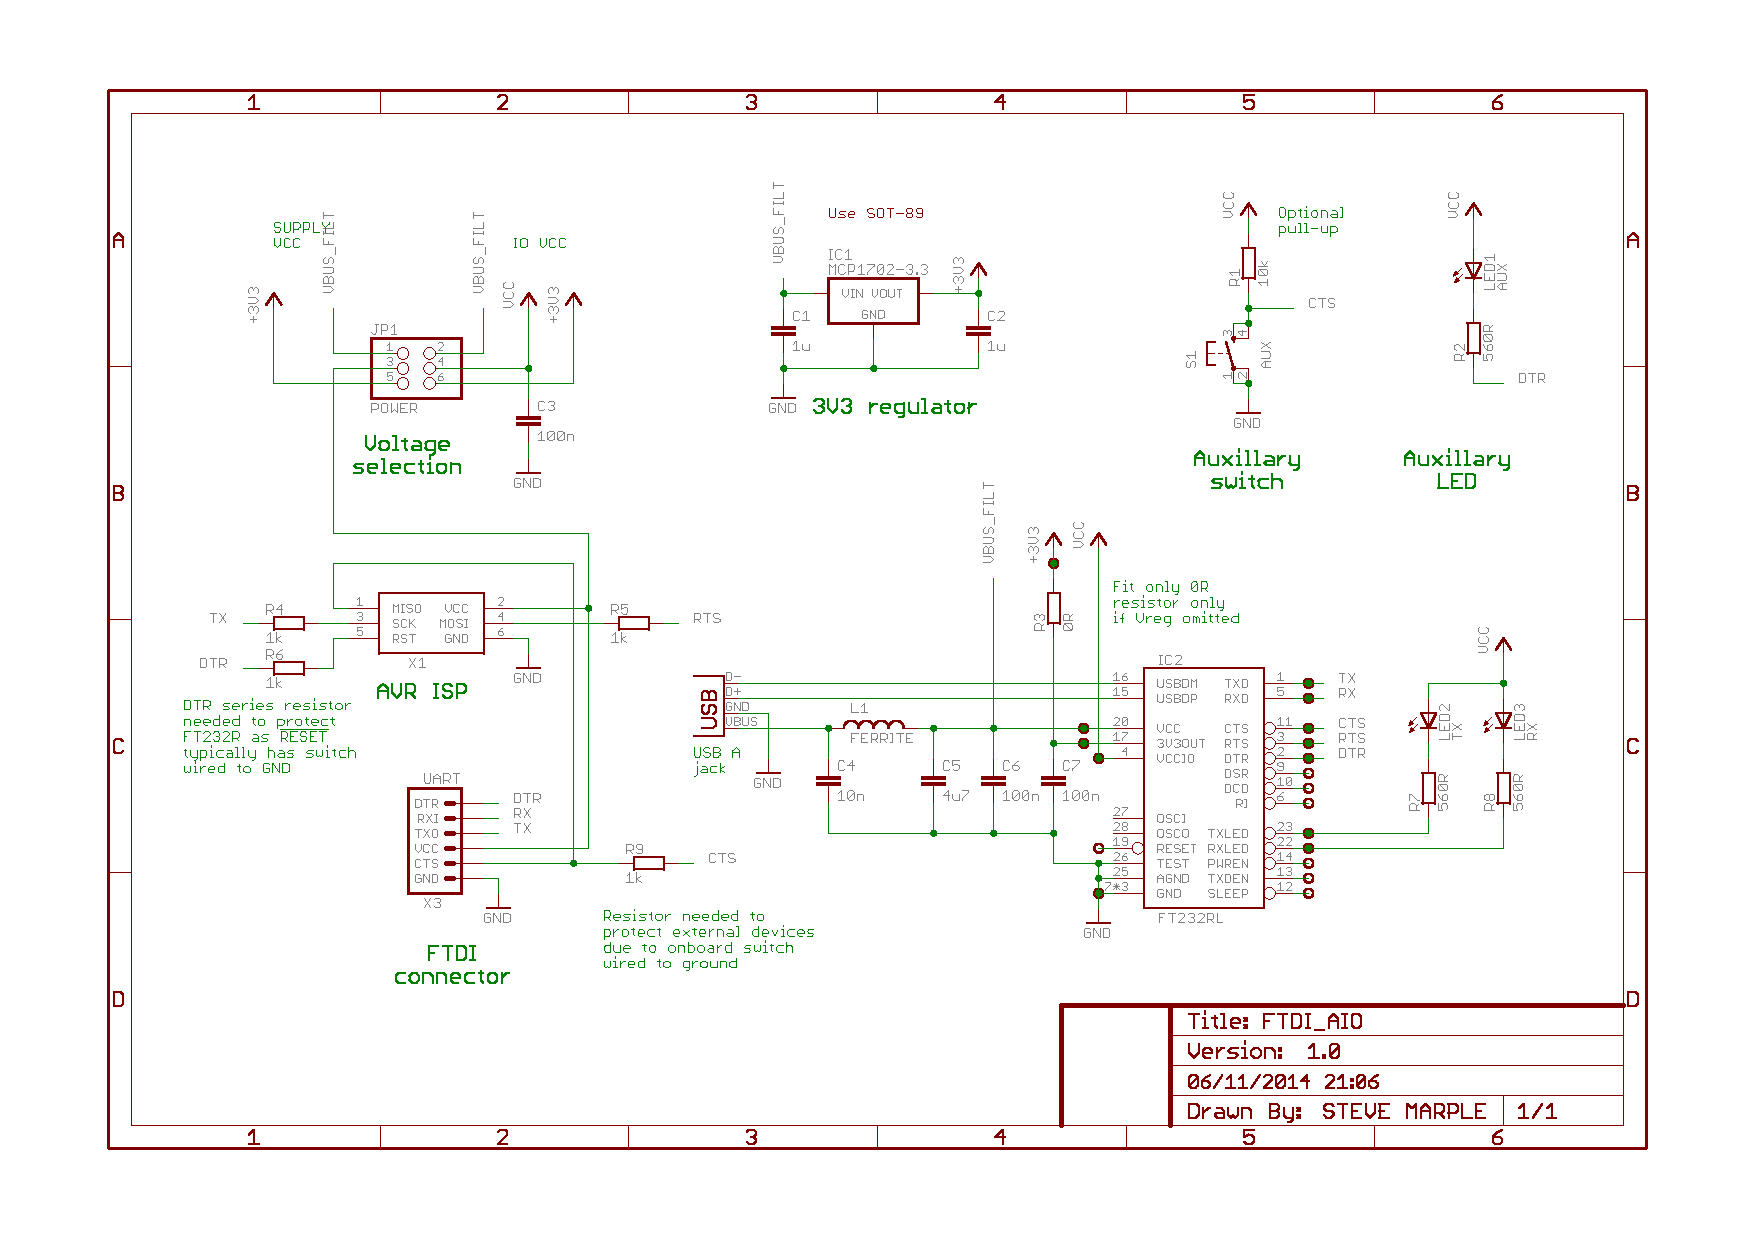
\includegraphics[keepaspectratio,width=28cm,height=16cm]{%
      images/FTDI_AIO_sch}
     \caption{FTDI all-in-one v.~1.0 circuit diagram.}
  \end{figure}
\end{landscape}

\end{document}

